%%%%%%%%%%%%%%%%%%%%%%%%%%%%%%%%%%%%%%%%%%%%%%%%%%%%%%%%%%%%%%%%%%%%%%
% How to use writeLaTeX: 
%
% You edit the source code here on the left, and the preview on the
% right shows you the result within a few seconds.
%
% Bookmark this page and share the URL with your co-authors. They can
% edit at the same time!
%
% You can upload figures, bibliographies, custom classes and
% styles using the files menu.
%
%%%%%%%%%%%%%%%%%%%%%%%%%%%%%%%%%%%%%%%%%%%%%%%%%%%%%%%%%%%%%%%%%%%%%%

\documentclass[12pt]{article}

\usepackage{sbc-template}

\usepackage{graphicx,url}

%\usepackage[brazil]{babel}   
\usepackage[utf8]{inputenc}  
\usepackage[lined,algonl,ruled]{algorithm2e}
\usepackage{amsmath}
\usepackage{multirow}

     
\sloppy

\title{Compiladores - Trabalho Prático }

\author{Paulo Viana Bicalho\inst{1}}


\address{Departamento de Ciência da Computação -- Universidade Federal de minas gerais
  (UFMG)\\
  \email{\{p.bicalho\}@dcc.ufmg.br}
}

\begin{document} 

\maketitle

     
\begin{resumo} 
  Este relatório descreve a implementação de um compilador de uma determinada linguagem para \textit{bytecode} Java. O processo de desenvolvimento foi dividido em três partes principais: Desenvolvimento do \textit{front-end}, Desenvolvimento do \textit{back-end}, e Integração de ambos. O principal objetivo deste trabalho é o de praticar conceitos e técnicas estudados na disciplina de Compiladores. Para avaliar o compilador desenvolvido, foram realizados uma série de testes e os resultados obtidos ficaram dentre os esperados.
\end{resumo}


\section{Introdução}

Computadores e máquinas computacionais no geral, são capazes de executar uma série de comandos para executar determinadas tarefas.
Para tanto, eles possuem um conjunto de instruções, onde cada instrução desempenha uma tarefa especifica. O grande problema, é que de maneira geral, estas instruções são pouco intuitivas, o que torna difícil a arte de programação. Para solucionar tal problema, surgiram as linguagens de programação. Uma linguagem de programação aumenta o nível de abstração das instruções da máquina, disponibilizando comandos e procedimentos que possuem mair valor semântico.

Como advento destas linguagens, foi então, necessário desenvolver um tipo de programa que seja capaz de converter ou traduzir um programa fonte desta linguagem mais abstrata, para um programa objeto da linguagem alvo. Tais programas são chamados de compiladores e são vitais nos dias atuais para o sucesso da computação no geral.

Este trabalho possui como objetivo, implementar um compilador de uma determinada linguagem para bytecode da JVM (\textit{Java Virtual Machine}). O desenvolvimento foi dividido em três partes principais:

\begin{itemize}
	\item \textit{Front-end}: Responsável por realizar a análise do programa fonte e geração de uma forma intermediária do programa;
	\item \textit{Back-end}: Responsável pela síntese, recebe como entrada a saída do \textit{front-end} e constrói o programa objeto;
	\item Integração: Integra as duas partes anteriores;
\end{itemize}

\section{A Gramática}
\label{sec:gram}

A gramática da linguagem de origem é dada na figura \ref{fig:gram}.

%----------AMBIENTE DE FIGURA-----------------
\begin{figure}[h!]
\centering
%------------PRIMEIRA FIGURA------------------
\begin{minipage}[b]{0.77\linewidth}
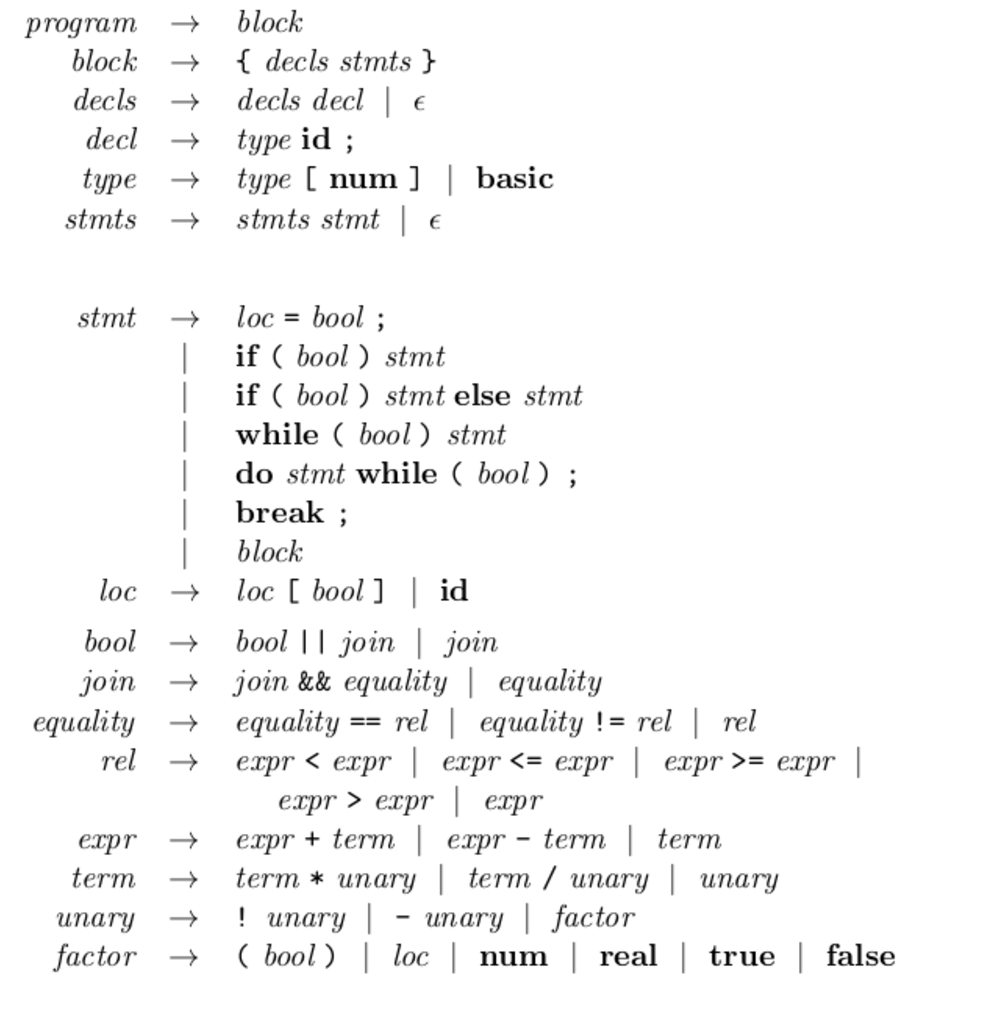
\includegraphics[width=\linewidth]{gram}
\end{minipage}
%---------------------------------------------
\caption{Gramática}
\label{fig:gram}
\end{figure}
%---------------------------------------------

\section{\textit{Front-End}}
\label{sec:frontend}

A parte da análise geralmente é subdividida em três fases: Análise Léxica, Análise Sintática e Análise Semântica. Cada uma destas análises possui um propósito específico que se complementam. A figura \ref{fig:frontend} exibe uma decomposição típica do \textit{front-end} em fases

%----------AMBIENTE DE FIGURA-----------------
\begin{figure}[h!]
\centering
%------------PRIMEIRA FIGURA------------------
\begin{minipage}[b]{0.77\linewidth}
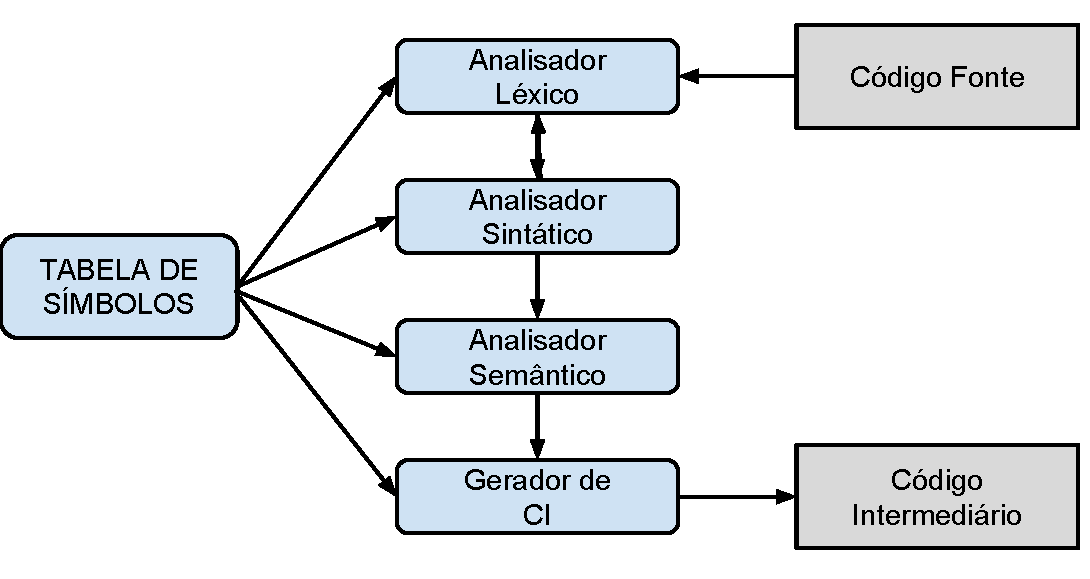
\includegraphics[width=\linewidth]{frontend}
\end{minipage}

\caption{Fases do \textit{Front-End} de um compilador}
\label{fig:frontend}
\end{figure}
%---------------------------------------------

\subsection{Análise Léxica}

O Analisador Léxico é a única parte do compilador que tem acesso direto ao código fonte original. Seu principal papel é o de realizar a leitura de tal arquivo, agrupando sequências de caracteres que são de alguma forma significativas. Estas sequências, chamadas de lexemas, são palavras que possuem algum valor semântico associados à elas.

O Analisador Léxico deve garantir que todos os lexemas lidos pertencem à gramática da linguagem fonte e deve ser capaz de associar a cada lexema o tipo deste. Assim, para cada lexema o analisador produz como saída um token na forma:

\begin{center}{
\textit{$< tipo-token,lexema >$}}
\end{center}

O Analisador desenvolvido neste trabalho realiza casamento de padrões para extrair os lexemas e associar tipos a estes. A implementação foi baseada na secção 2.6 do livro texto da disciplina \cite{Aho:2006:CPT:1177220}.

\subsection{Análise Sintática}

O principal papel deste Analisador é o de utilizar os \textit{tokens} produzidos pelo Analisador Léxico e criar uma árvore de derivação sintática. A construção desta árvore é realizada seguindo as regras de produções da gramática e geralmente cada nó desta árvore esta associada à uma operação e cada filho deste nó os operandos.

Esta análise pode ser realizada utilizando diversas técnicas diferentes. Estas técnicas podem ser agrupadas em dois grandes grupos:

\begin{itemize}
\item \textit{Top-Down}: As técnicas que utilizam esta abordagem iniciam a construção da derivação sintática a partir das regras iniciais da gramática fazendo o refinamento a cada passo.

\item \textit{Bottom-Up}: A construção é realizada inicialmente pelos nós inferiores da árvore aumentando o nível a cada etapa.
\end{itemize}

Neste trabalho foi implementado um Analisador Sintático preditivo (\textit{Top-Down}) conforme descrito na seção 2.4 do livro texto \cite{Aho:2006:CPT:1177220}.

\subsection{Análise Semântica}

Durante as etapas da Análise Léxica e Sintática os lexemas, seus tipos e algumas outras informações pertinentes como tamanho de \textit{arrays} são armazenados na tabela de símbolos. O Analisador Semântico utiliza destes valores para validar as operações executados no código fonte original.

Nesta verificação ocorre principalmente a checagem de tipos, que verifica se os operandos das operações são válidos para a mesma.

O Analisador Semântico desenvolvido neste trabalho foi baseado na descrição da secção 2.6 do livro texto da disciplina \cite{Aho:2006:CPT:1177220}.

\subsection{Geração de Código Intermediário}

Realizadas as análises, ou juntamente com elas, o \textit{Front-End} é capaz de gerar um código intermediário (CI) que possui a mesma semântica que o código fonte original.

A grande utilidade do CI é o de permitir a separação e a independência entre o \textit{Front-End} e o \textit{Back-End}. Além disso, como o geralmente este tipo de código é muito simples, facilita o processo de otimização.

O CI desenvolvido é um CI de três endereços baseado na seção 2.8 do livro texto \cite{Aho:2006:CPT:1177220}.

Para facilitar o processo de criação do \textit{back-end}, foram utilizadas algumas convenções para a construção do código intermediário

\begin{enumerate}
\item Todas as variáves não temporárias são representadas na forma: var\_$type(x)$ onde $type$ é o tipo da variável e $x$ o identificador da mesma;

\item Todas as constantes são identificadas da seguinte forma: var\_ $ type( $const(x)) onde $type$ representa o tipo da variável, $x$ é o identificador e $const$ informa que é alguma constante;

\item As operações aritméticas também são diferenciadas de acordo com o tipo da variável de destino.;

\item As variáveis temporáriras são nomeadas da seguinte forma: $t1, t2, t3, ..., tn$;

\end{enumerate}

\subsection{Código}

O Código do \textit{Front-End} foi desenvolvido em \textbf{C++ 11} em um ambiente Unix e se encontra da pasta \textit{front} do anexo enviado com esta documentação. A estruturação foi baseada nos exemplos do livro texto e o código foi organizados em sub-pastas sendo:

\begin{itemize}
\item inter: Geração de Código Intermediário / Analise Semântica;
\item lexer: Analisador Léxico;
\item parser: Analise Sintática;
\item symbols: Tabela de simbolos;
\end{itemize}

Um Makefile acompanha o código para facilitar a compilação. A chamada do executável do \textit{front-end} espera como parâmetro o arquivo fonte e deve ser realizada da seguinte forma:

\begin{verbatim}
 ./frontend arquivo_fonte
\end{verbatim}

A saida do programa é a saida padrão e caso seja necessário, pode ser redirecionada através do comando $>$ do bash;

\begin{verbatim}
 ./frontend arquivo_fonte.p > arquivo_saida.i
\end{verbatim}

\section{\textit{Back-End}}
\label{sec:backend}

O \textit{Back-End} desenvolvido recebe como entrada, a saida do \textit{Front-End} e realiza o mapeamento deste código em bytecode da JVM.

A JVM é uma máquina de pilha e possui um grande número de instruções. Muitas destas instruções não foram utilizadas pois a gramática da linguagem fonte é muito simples.

Como referencia de estudo das instruções, foi utilizado a wikipédia principalmente a página \url{http://en.wikipedia.org/wiki/Java_bytecode_instruction_listings}.

\subsection{Código}

O código do \textit{Back-End} também foi desenvolvido em \textbf{C++ 11} em um ambiente Unix e se encontra na pasta \textit{back}. Como a quantidade arquivos necessários é muito menor que a do \textit{Front-End}, não foi necessário a estruturação em sub-pastas.

Um Makefile acompanha o código e a chamada do executável deve ser executada da seguinte forma:

\begin{verbatim}
 ./backend arquivo_intermediario.i
\end{verbatim}

O parâmetro esperado é um arquivo com um código na representação intermediária (saída do \textit{Front-End}). A saída é a saída padrão do sistema mas pode ser redirecionada.

\begin{verbatim}
 ./backend arquivo_intermediario.i > arquivo_saida.jvm
\end{verbatim}


\section{Integração}

A integração das duas etapas foi realizada na pasta principal do anexo enviado e possui somente um arquivo que realiza a chamada do \textit{Front-End} seguido pela chamada do \textit{Back-End}.

O executável espera três parâmetros: Arquivo fonte, Arquivo de saída do \textit{Front-End}, Arquivo de saída do \textit{Back-End}.

\begin{verbatim}
 ./pauloCompiler arquivo_font.p arquivo_ci.i arquivo_final.jvm
\end{verbatim}

Um Makefile acompanha o código para facilitar a compilação.


\section{Testes}

Para avaliar o compilador proposto foram realizados vários testes. Como dito anteriormente, tanto o \textit{Front-End}, o \textit{Back-End} quanto o compilador encontrado possuem um Makefile que acompanha o código. Tal Makefile contém uma seção de testes que pode ser invocada da seguinte maneira

\begin{verbatim}
 make test
\end{verbatim}

Ao realizar tal chamada, os arquivos dentro da pasta $test_in$ são passados como parâmetro de entrada para o executável e as saídas são armazenadas na pasta $test_out$.


\section{Conclusão}

Este relatório discutiu a implementação de um compilador para uma determinada gramática. Tal compilador foi dividido em duas grandes partes: \textit{Front-End} e \textit{Back-End}. O \textit{Front-End} é o responsável de realizar as análises no código fonte e gerar uma representação intermediária do mesmo enquanto o \textit{Back-End} deve converter este código intermediário em bytecode da JVM.

A compilador foi testado com uma gama de arquivos de teste e os resultados obtidos ficaram dentre os esperados. Desta forma, este trabalho cumpriu seus objetivos pois proporcionou ao aluno vivenciar a experiência e as dificuldades de se projetar e implementar um compilador.


\bibliographystyle{sbc}
\bibliography{sbc-template}

\end{document}
